\begin{table*}[htbp]
    \centering  
    \caption{Representative basic and advanced abilities and corresponding representative datasets for evaluating.}
    \footnotesize
    \renewcommand\tabcolsep{2.5pt}
    \begin{tabular}{cccc}
        \toprule
        \textbf{Level} & \textbf{Ability} & \textbf{Task} & \textbf{Dataset} \\
        \midrule
        \multirow{27}{*}{Basic} & \multirow{6}{*}{Language Generation}    &Language Modeling             &Penn Treebank~\cite{Marcus-CL-1993-Building}, WikiText-103~\cite{Merity-ICLR-2017-Pointer}, the Pile~\cite{Gao-arxiv-2021-Pile}, LAMBADA~\cite{Paperno-ACL-2016-LAMBADA} \\ 
        \addlinespace
                                            &    &\multirow{3}{*}{Conditional Text Generation}   & WMT'14,16,19,20,21,22~\cite{Bojar-WMT-2014-Findings,Bojar-WMT-2016-Findings,Barrault-WMT-2019-Findings,Barrault-WMT-2020-Findings,Akhbardeh-WMT-2021-Findings,Kocmi-WMT-2022-Findings}, Flores-101~\cite{Goyal-TACL-2022-The}, DiaBLa~\cite{Bawden-journal-2021-DiaBLa}, \\ 
                                              &  & &  
                                                CNN/DailyMail~\cite{Nallapati-acl-2016-Abstractive}, XSum~\cite{Naryan-EMNLP-2018-XSUM}, WikiLingua~\cite{Ladhak-EMNLP-2020-WikiLingua}\\
                                            & & & OpenDialKG~\cite{Moon-ACL-2019-OpenDialKG} \\
                                                
                                                 \addlinespace
                                             &   &\multirow{2}{*}{Code Synthesis}                & APPS~\cite{Hendrycks-nips-2021-Measuring}, HumanEval~\cite{Chen-arxiv-2021-evaluating}, MBPP~\cite{Austin-arxiv-2021-Program}, CodeContest~\cite{Li-Science-2022-AlphaCode},
                                                MTPB~\cite{nijkamp-arxiv-2022-Codegen},
                                                \\ 
                                             &   &   &
                                                DS-1000~\cite{Lai-arxiv-2022-DS}, ODEX~\cite{Wang-arxiv-2022-Execution} \\
                                                \cmidrule(r){2-4}
        &\multirow{9}{*}{Knowledge Utilization}  
            &\multirow{3}{*}{Closed-Book QA}                &  
                Natural Questions~\cite{Kwiatkowski-ACL-2019-Natural}, 
                ARC~\cite{Clark-arxiv-2018-Think},  
                TruthfulQA~\cite{Lin-ACL-2022-TruthfulQA}, 
                Web Questions~\cite{Berant-EMNLP-2013-Semantic},\\
          &  &           & 
                TriviaQA~\cite{Joshi-ACL-2017-TriviaQA}, 
                PIQA~\cite{Bisk-AAAI-2020-PIQA}, 
                LC-quad2.0~\cite{Dubey-ISWC-2019-LC}, 
                GrailQA~\cite{Gu-WWW-2021-Beyond}, 
                KQApro~\cite{Cao-ACL-2022-KQA},\\ 
          &  &           &
                CWQ~\cite{Hu-COLING-2022-Logical}, 
                MKQA~\cite{Longpre-TACL-2021-MKQA}, 
                ScienceQA~\cite{Saikh-IJDL-2022-ScienceQA} \\
            \addlinespace
         &   &\multirow{3}{*}{Open-Book QA}                  &  
                Natural Questions~\cite{Kwiatkowski-ACL-2019-Natural}, 
                OpenBookQA~\cite{Mihaylov-EMNLP-2018-Can}, 
                ARC~\cite{Clark-arxiv-2018-Think}, 
                TriviaQA~\cite{Joshi-ACL-2017-TriviaQA}, \\
          &  &           &  
                 Web Questions~\cite{Berant-EMNLP-2013-Semantic},
                MS MARCO~\cite{Nguyen-NIPS-2016-MS}, 
                QASC~\cite{Khot-AAAI-2020-QASC}, 
                SQuAD~\cite{Rajpurkar-EMNLP-2016-SQuAD}, 
                \\
        &  &           &  
                WikiMovies~\cite{Miller-EMNLP-2016-Key} \\
            \addlinespace
          &  &\multirow{2}{*}{Knowledge Completion}          & 
                WikiFact~\cite{Goodrich-KDD-2019-Assessing}, 
                FB15k-237~\cite{Toutanova-CVSC-2015-Observed}, 
                Freebase~\cite{Bollacker-SIGMOD-2008-Freebase}, 
                WN18RR~\cite{Dettmers-AAAI-2018-Convolutional}, \\
          &  &           &
                WordNet~\cite{Miller-Commun-1995-WordNet},
                LAMA~\cite{Petroni-EMNLP-2019-Language}, 
                YAGO3-10~\cite{Mahdisoltani-CIDR-2015-YAGO3}, 
                YAGO~\cite{Suchanek-WWW-2007-Yago}\\ 
        \cmidrule(r){2-4}
        & \multirow{12}{*}{Complex Reasoning}      &\multirow{4}{*}{Knowledge Reasoning}           &  CSQA~\cite{Talmor-naacl-2019-CommonsenseQA}, StrategyQA~\cite{Geva-tacl-2021-Did}, HotpotQA~\cite{yang-2018-acl-HotpotQA}, ARC~\cite{Clark-arxiv-2018-Think}, BoolQ~\cite{Clark-naacl-2019-BoolQ},  \\ 
                                              &  &   &
                                                PIQA~\cite{Bisk-AAAI-2020-PIQA},
                                                SIQA~\cite{Sap-arxiv-2019-SocialIQA}, HellaSwag~\cite{Zellers-acl-2019-HellaSwag}, WinoGrande~\cite{Sakaguchi-aaai-2020-WinoGrande}, 
                                                COPA~\cite{Roemmele-aaai-2011-Choice}, \\
                                             &  &   &
                                                OpenBookQA~\cite{Mihaylov-EMNLP-2018-Can},
                                                 ScienceQA~\cite{Saikh-IJDL-2022-ScienceQA}, proScript~\cite{Sakaguchi-acl-2021-proScript}, ProPara~\cite{Dalvi-acl-2018-Tracking},  \\ 
                                              &  &   &
                                                ExplaGraphs~\cite{Saha-acl-2021-ExplaGraphs},
                                                ProofWriter~\cite{Tafjord-acl-2021-ProofWriter},  EntailmentBank~\cite{Dalvi-acl-2021-Explaining},  \\ 
                                            &  &   &
                                                ProOntoQA~\cite{Saparov-arxiv-2022-Language}  \\ 
                                                \addlinespace
                                             &   &\multirow{3}{*}{Symbolic Reasoning}            & 
                                                CoinFlip~\cite{Wei-arxiv-2022-chain}, ReverseList~\cite{Wei-arxiv-2022-chain},  LastLetter~\cite{Wei-arxiv-2022-chain}, Boolean Assignment~\cite{Anil-arxiv-2022-Exploring},
                                                \\
                                             &   &    &
                                                Parity~\cite{Anil-arxiv-2022-Exploring}, Colored Object~\cite{Srivastava-arxiv-2022-Beyond}, Penguins in a Table~\cite{Srivastava-arxiv-2022-Beyond},   \\
                                             &   &   &
                                                Repeat Copy~\cite{Gao-arxiv-2022-PAL}, Object Counting~\cite{Gao-arxiv-2022-PAL}  \\
                                                \addlinespace
                                             &   &\multirow{3}{*}{Mathematical Reasoning}        &  MATH~\cite{Hendrycks-ICLR-2021-Measuring}, GSM8k~\cite{Cobbe-arxiv-2021-Training}, SVAMP~\cite{Patel-NAACL-2021-Are}, MultiArith~\cite{Roy-acl-2015-Solving}, ASDiv~\cite{Miao-ACL-2020-A}, \\
                                             &   &  &
                                                MathQA~\cite{Amini-acl-2019-MathQA}, 
                                                AQUA-RAT~\cite{Ling-acl-2017-Program}, MAWPS~\cite{Koncel-NAACL-2016-MAWPS}, DROP~\cite{Dua-NAACL-2019-DROP},  \\
                                             &   &  & 
                                                NaturalProofs~\cite{Welleck-NIPS-2021-NaturalProofs},
                                                PISA~\cite{Jiang-AITP-2021-LISA},
                                                miniF2F~\cite{Zheng-ICLR-2022-miniF2F}, ProofNet~\cite{Azerbayev-arxiv-2023-ProofNet}  \\
                                                \midrule
    \multirow{18}{*}{Advanced} & \multirow{5}{*}{Human Alignment}    & Honestness             &TruthfulQA~\cite{Lin-ACL-2022-TruthfulQA}, HaluEval~\cite{Li-arxiv-2023-HaluEval} \\
        \addlinespace
        & & Helpfulness             & HH-RLHF~\cite{Bai-arxiv-2022-Training} \\
        \addlinespace
        & & \multirow{2}{*}{Harmlessness}             & HH-RLHF~\cite{Bai-arxiv-2022-Training}, Crows-Pairs~\cite{Nangia-EMNLP-2020-CrowS} \\
        & & & WinoGender~\cite{Rudinger-NAACL-2018-Gender}, RealToxicityPrompts~\cite{Gehman-2023-arxiv-RealToxicityPrompts} \\
        \cmidrule(r){2-4}
        & \multirow{4}{*}{\makecell[c]{Interaction with \\ External Environment}}    &       \multirow{1}{*}  Household       & VirtualHome~\cite{Puig-CVPR-2018-VirtualHome}, BEHAVIOR~\cite{Srivastava-CoRL-2021-BEHAVIOR}, ALFRED~\cite{Shridhar-CVPR-2020-ALFRED},ALFWorld~\cite{Shridhar-2021-iclr-ALFWorld} \\
        \addlinespace
        & &       \multirow{1}{*}  Website Environment   & WebShop~\cite{Yao-2022-nips-WebShop}, Mind2Web~\cite{Deng-2023-arxiv-Mind2Web}  \\
        \addlinespace
        & &       \multirow{1}{*}  Open World       &MineRL~\cite{Guss-2019-ijcai-MineRL}, MineDojo~\cite{Fan-2022-nips-minedojo} \\
        \cmidrule(r){2-4}
        &  \multirow{8}{*}{Tool Manipulation}    & \multirow{1}{*} Search Engine             & HotpotQA~\cite{yang-2018-acl-HotpotQA}, TriviaQA~\cite{Joshi-ACL-2017-TriviaQA}, Natural Questions~\cite{Kwiatkowski-ACL-2019-Natural} \\
        \addlinespace
        & & \multirow{1}{*} Code Executor             & GSM8k~\cite{Cobbe-arxiv-2021-Training}, TabMWP~\cite{Lu-2022-arxiv-Dynamic}, Date Understanding~\cite{Srivastava-arxiv-2022-Beyond} \\
        \addlinespace
        & & \multirow{1}{*} Calculator             & GSM8k~\cite{Cobbe-arxiv-2021-Training}, MATH~\cite{Hendrycks-ICLR-2021-Measuring}, CARP~\cite{Zhang-2023-arxiv-Evaluating} \\
        \addlinespace
        & & \multirow{1}{*} Model Interface             & GPT4Tools~\cite{yang-2023-arxiv-GPT4Tools}, Gorilla~\cite{Patil-2023-arxiv-Gorilla} \\
        \addlinespace
        & & \multirow{2}{*}{Data Interface}             & WebQSP~\cite{Yih-2016-acl-The}, MetaQA~\cite{Puerto-2023-eacl-MetaQA}, WTQ~\cite{Pasupat-2015-acl-Compositional} \\
        & & & WikiSQL~\cite{Zhang-2017-arxiv-Seq2SQL}, TabFact~\cite{Chen-2020-iclr-TabFact}, Spider~\cite{Yu-2018-emnlp-Spider} \\
        \addlinespace
        \bottomrule
    \end{tabular}
    \label{tab:dataset}
\end{table*}


\subsection{Basic Ability}\label{sec:basicability}
In this part, we mainly focus on three basic types of ability evaluation for LLMs, \ie language generation, knowledge utilization, and complex reasoning. 
It is noted that we do not intend to have complete coverage of all the related tasks, but instead only focus on the most widely discussed or studied tasks for LLMs.  Next, we introduce these tasks in detail.  


\subsubsection{Language Generation}
\label{sec-langauge-generation}
According to the task definition, existing tasks about language generation can be roughly categorized into language modeling, conditional text generation, and code synthesis tasks. Note that code synthesis is not a typical NLP task, we include it for discussion because it can be directly solved by a number of LLMs (trained on code data) in a similar generation approach as natural language text.   

\paratitle{Language Modeling.}
As the most fundamental ability of LLMs, \emph{language modeling} aims  to predict the next token based on the previous tokens~\cite{Bengio-JMLR-2003-A}, which mainly focuses on the capacity of basic language understanding and generation.  For evaluating such an ability, typical language modeling datasets that existing work uses include Penn Treebank~\cite{Marcus-CL-1993-Building}, WikiText-103~\cite{Merity-ICLR-2017-Pointer}, and the Pile~\cite{Gao-arxiv-2021-Pile}, where the metric of \emph{perplexity} is commonly used for evaluating the model performance under the zero-shot setting. 
Empirical studies~\cite{Brown-NeurIPS-2020-Language,Zeng-arxiv-2022-GLM} show that LLMs bring substantial performance gains over the previous state-of-the-art methods on these evaluation datasets. 
To better test the modeling capacity of long-range dependencies in text, the LAMBADA dataset~\cite{Paperno-ACL-2016-LAMBADA} has been introduced, where LLMs are required to predict the last word of sentences based on a paragraph of context.
Then, the accuracy and perplexity of the predicted last words are employed  to evaluate LLMs. 
As shown in existing work, the performance on the language modeling tasks typically follows the scaling law~\cite{Kaplan-arxiv-2020-Scaling}, which means that scaling language models would improve the accuracy and reduce the perplexity.

\paratitle{Conditional Text Generation.}
As an important topic in language generation, conditional text generation~\cite{Li-IJCAI-2021-Pretrained} focuses on generating texts satisfying specific task demands based on the given conditions, typically including machine translation~\cite{Bahdanau-ICLR-2015-Neural}, text summarization~\cite{Nallapati-acl-2016-Abstractive}, and question answering~\cite{Berant-EMNLP-2013-Semantic}.
{To measure the quality of the generated text, automatic metrics (\eg Accuracy, BLEU~\cite{Papineni-acl-2002-bleu} and ROUGE~\cite{lin-acl-2004-rouge}) and human ratings have been typically used for evaluating the performance. } 
Due to the powerful language generation capabilities, LLMs have achieved remarkable performance on existing datasets and benchmarks.
{For instance, GPT-4 exhibits comparable performance as commercial translation products, {even for the translation task of languages that are with significant linguistic distance~\cite{Jiao-arxiv-2023-mt}.}
On news summarization tasks~(\ie CNN/DM and XSUM), LLMs also demonstrate comparable performance with human freelance writers~\cite{Zhang-2023-arxiv-Benchmarking}.
Despite the rapid progress on model capacity, there are increasing concerns on the feasibility of existing automatic metrics to faithfully assess the performance of LLMs in conditional text generation tasks~\cite{Zhang-2023-arxiv-Benchmarking,Goyal-2023-arxiv-News,Gehrmann-2022-arxiv-Repairing}. 
As the alternatives to automatic metrics, recent studies also propose to incorporate LLMs as generation evaluators to examine the quality of the generated content~\cite{Wang-2023-arxiv-Is,Liu-2023-arxiv-G-Eval,vicuna2023}. 
Moreover, researchers also explore more challenging language generation tasks for LLMs, such as  structured data generation~\cite{Jiang-2023-arxiv-StructGPT} and long text generation~\cite{Yang-EMNLP-2022-Re3,OpenAI-OpenAI-2023-GPT-4,Zhou-2023-arxiv-RecurrentGPT}.}



\paratitle{Code Synthesis.}
In addition to generating high-quality natural language text, existing LLMs also show strong abilities to generate {formal language, especially  computer programs (\ie code)} that satisfy specific conditions, called \emph{code synthesis}~\cite{Gulwani-Found-2017-Program}. 
Unlike natural language generation, as the generated code can be directly checked by execution with corresponding compilers or interpreters, existing work mostly evaluates the quality of the generated code from LLMs by calculating the pass rate against the test cases, \ie pass@$k$\footnote{Given $k$ programs generated by the LLM, pass@$k$ is computed as 1 when at least one program passes all test cases, or else 0}. %
Recently, several code benchmarks focusing on functional correctness are proposed to assess the code synthesis abilities of LLMs, such as APPS~\cite{Hendrycks-nips-2021-Measuring}, HumanEval~\cite{Chen-arxiv-2021-evaluating}, and MBPP~\cite{Austin-arxiv-2021-Program}. 
Typically, they consist of diverse programming problems, with text specification and test cases for correctness checking. 
To improve such an ability, it is key to fine-tuning (or pre-training) LLMs on code data, which can effectively adapt LLMs to code synthesis tasks~\cite{nijkamp-arxiv-2022-Codegen}.
{In addition, existing work  has proposed new strategies to generate code, \eg sampling multiple candidate solutions~\cite{Austin-arxiv-2021-Program} and planning-guided decoding~\cite{Zhang-ICLR-2023-Planning}, which can be considered as the imitation of bug-fixing and code-planning processes by  programmers.}
Impressively,  LLMs have recently shown competitive performance with humans by achieving a ranking of the top 28\% among users on the programming contest platform Codeforces~\cite{Li-Science-2022-AlphaCode}. 
Further, GitHub Copilot has been released to assist programming in coding IDEs (\eg Visual Studio and JetBrains IDEs), which can support  a variety of  languages including Python, JavaScript, and Java. 
A viewpoint article entitled ``\emph{The End of Programming}''~\cite{Welsh-ACM-2023-The} in Communications of the ACM  has discussed the impact of AI programming in the field of computer science, emphasizing an important shift towards the highly adaptive LLM as a new atomic  unit of computation. 

\paratitle{Major Issues.} Although LLMs have achieved splendid performance in generating human-like text, they are susceptible to suffering from two major issues in language generation as discussed below.

$\bullet$ \emph{Unreliable generation evaluation.}
\label{sec:generation-eval}
With the advancement of  language generation ability of LLMs, existing studies find that 
the generated texts from LLMs have reached a comparable quality to the reference texts on a variety of text  generation tasks. However, due to the intrinsic weakness of existing evaluation benchmarks, there exists pronounced inconsistency between human evaluation and automatic reference-based metrics~\cite{Zhang-2023-arxiv-Benchmarking,Goyal-2023-arxiv-News,Gehrmann-2022-arxiv-Repairing,Bang-arxiv-2023-A}. For example, 
in OpenDialKG~\cite{Moon-ACL-2019-OpenDialKG}, ChatGPT underperforms a fine-tuned GPT-2 on BLEU and ROUGE-L metrics, while earning more favor from human judgment~\cite{Bang-arxiv-2023-A}. Furthermore, existing work argues that even human evaluation may  not be robust enough~\cite{Goyal-2023-arxiv-News,Zhang-2023-arxiv-Benchmarking,Liu-arxiv-2022-Revisiting,Fabri-2021-tacl-SummEval}.
In some cases, it is difficult to achieve a high level of consensus among human annotators~\cite{Goyal-2023-arxiv-News}, and there is also a large gap between the annotation quality of crowdworkers and experts~\cite{Fabri-2021-tacl-SummEval,Liu-arxiv-2022-Revisiting}.
Thus, how to conduct reliable evaluation for language generation tasks in the era of LLMs has become a fundamental yet challenging research topic. 
Recently, increasing research work proposes to leverage LLMs to improve the evaluation quality of the generated texts.  
Specially, LLMs can be   used to improve the evaluation quality of existing metrics.
For example, Para-Ref~\cite{Tang-2023-arxiv-Not} augments various automatic metrics by leveraging LLMs to paraphrase existing references into semantically equivalent references with diverse expressions. 
Further, LLMs are widely employed as the evaluators of text generation in a reference-free manner, including evaluating a single prediction~\cite{Wang-2023-arxiv-Is,Liu-2023-arxiv-G-Eval,Wang-2023-arxiv-rethinking} or comparing several candidates~\cite{Gao-arxiv-2023-Human,Ji-2023-arxiv-Exploring,vicuna2023,Bai-2023-arxiv-Benchmarking}. 
Nevertheless, LLMs may expose bias (\eg order bias or preference for LLM-generated texts over human-written texts) as language generation evaluators, demonstrating disparities when compared to human evaluation~\cite{Liu-2023-arxiv-Evaluate,Liu-2023-arxiv-G-Eval,Wang-2023-arxiv-Large}. 

\begin{center}
\begin{tcolorbox}[colback=blue!5!white,colframe=blue!55!black,width=0.46\textwidth,title={Unreliable Generation Evaluation}]
LLMs have been capable of generating texts with a comparable quality to human-written texts, which however might be underestimated by automatic reference-based metrics. %
As an alternative evaluation approach, 
LLMs can serve as language generation evaluators to evaluate a single text, compare multiple candidates, and improve existing metrics. However, this evaluation approach still needs more inspections and examinations in real-world tasks.  
\end{tcolorbox}
\end{center}



$\bullet$ {\emph{Underperforming specialized generation}}. Although LLMs have learned general language patterns to generate coherent text, 
their proficiency in generation might be constrained when dealing  with a specialized domain or task. %
{For instance, a language model that has been trained on general web articles may face challenges when generating a medical report  which involves many medical jargon and methods.} 
Intuitively, domain knowledge should be critical for model specialization. However, it is not easy to inject such specialized knowledge into LLMs.   
As discussed in recent analyses~\cite{FU-blog-2022-how,Ye-arxiv-2023-A}, when LLMs are trained to exhibit some specific ability that allows them to excel in some areas, they might struggle in others. Such an issue is related to \emph{catastrophic forgetting}~\cite{Michael-Psychology-1989-Catastrophic, Kemker-AAAI-2018-Measuring} in training neural networks, which refers to the conflict phenomenon of integrating new and old knowledge.  
Similar cases also occur in human alignment of LLMs, where ``\emph{alignment tax}''~\cite{Ouyang-arxiv-2022-Training} (\eg a potential loss in the in-context learning  ability) has to be paid for aligning to human values and needs.  
{
Moreover, due to the limitations of sequence modeling architecture, LLMs still face challenges in the understanding and generation of structured data. Consequently, they often fall behind task-specific models on complex structured data tasks, such as knowledge-base question answering and semantic parsing~\cite{Xie-EMNLP-2022-UnifiedSKG,Jiang-2023-arxiv-StructGPT}.
}
Therefore, it is important to develop effective model specialization methods  that can flexibly adapt LLMs to various task scenarios,  meanwhile retaining the original abilities as possible. 

\begin{center}
\begin{tcolorbox}[colback=blue!5!white,colframe=blue!55!black,width=0.46\textwidth,title={Underperforming Specialized Generation}]
LLMs may fall short in mastering generation tasks that require domain-specific knowledge or generating structured data. It is non-trivial to inject specialized knowledge into LLMs, meanwhile maintaining the original abilities of LLMs.
\end{tcolorbox}
\end{center}

\begin{figure*}[h]
    \centering
        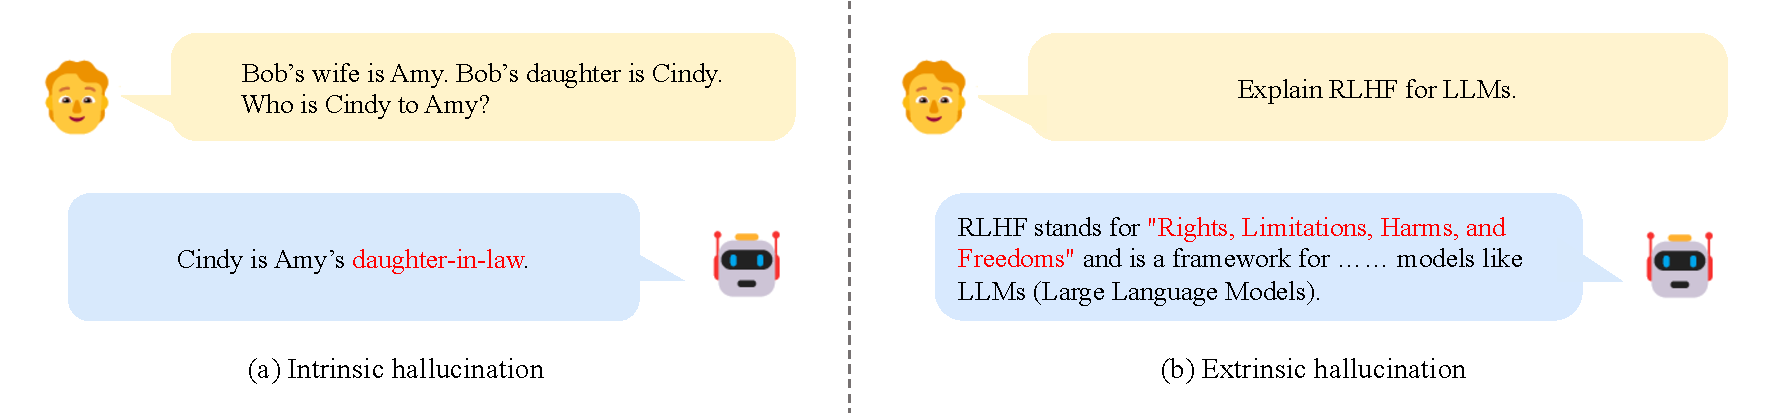
\includegraphics[width=1\textwidth]{images/hallucination.pdf}
    \caption{Examples of intrinsic and extrinsic hallucination for a public LLM (access date: March 19, 2023). As an example of intrinsic hallucination, the LLM gives a conflicting judgment about the relationship between Cindy and Amy, which  contradicts the input. 
{For extrinsic hallucination, in this example, the LLM seems to have an incorrect understanding of the meaning of RLHF (reinforcement learning from human feedback), though it can correctly understand the meaning of LLMs (in this context). } }
    \label{fig:hallucination}
\end{figure*}

\subsubsection{Knowledge Utilization}

Knowledge utilization is an important ability of intelligent systems to accomplish knowledge-intensive tasks (\eg commonsense question answering and fact completion) based on supporting factual evidence. 
Concretely, it requires LLMs to {properly utilize the rich factual knowledge from the pre-training corpus or retrieve external data when necessary.} 
In particular, question answering~(QA) and knowledge completion have been two commonly used tasks for evaluating this ability. 
According to the test tasks (question answering or knowledge completion) and evaluation settings (\emph{with} or \emph{without} external resources), we categorize existing knowledge utilization tasks into three types, namely closed-book QA, open-book QA\footnote{In this part, open-book QA refers to the QA tasks that require to extract and utilize useful information from external knowledge resources, as the antithesis of closed-book QA (only using the encoded information from  pre-training corpus). Note that there is a dataset  also named OpenBookQA~\cite{Mihaylov-EMNLP-2018-Can}, which  follows the settings of open-book QA tasks by extracting and utilizing  external science facts.}, and knowledge completion.



\paratitle{Closed-Book QA.}
Closed-book QA tasks~\cite{Roberts-EMNLP-2020-How} test the acquired factual knowledge of LLMs from the pre-training corpus, where LLMs should answer the question only based on the given context without using external resources. 
For evaluating this ability, there are  several datasets that can be leveraged, including  Natural Questions~\cite{Kwiatkowski-ACL-2019-Natural}, Web Questions~\cite{Berant-EMNLP-2013-Semantic}, and TriviaQA~\cite{Joshi-ACL-2017-TriviaQA}, %
{where the accuracy metric is widely adopted.}
Empirical results have revealed that  %
LLMs can perform well in this setting and even match the performance of state-of-the-art {open-domain} QA systems~\cite{Chowdhery-arxiv-2022-PaLM}.
Also, the performance of LLMs on closed-book QA tasks shows a scaling law pattern in terms of both model size and data size: 
scaling the parameters and training tokens can increase the capacity of LLMs and help them learn (or memorize) more knowledge from the pre-training data~\cite{Chowdhery-arxiv-2022-PaLM}. 
Further, under a similar parameter scale, LLMs with more pre-training data relevant to the evaluated tasks would achieve better performance~\cite{Nakano-arxiv-2021-WebGPT}. 
Also, the closed-book QA setting  provides a testbed for probing the accuracy of the factual knowledge encoded by LLMs. 
{However, as shown in existing work~\cite{Brown-NeurIPS-2020-Language}, LLMs might perform less well on QA tasks relying on fine-grained knowledge, even when it exists in the pre-training data.}






\paratitle{Open-Book QA.} %
Unlike closed-book QA, in open-book QA tasks, LLMs can extract useful evidence from the external knowledge base or document collections,  and then answer the question based on the extracted evidence~\cite{Izacard-arxiv-2022-Few, Guu-ICML-2020-Retrieval, Lewis-NeurIPS-2020-Retrieval,Lan-2021-arxiv-Complex}. 
{Typical open-book QA datasets (\eg Natural Questions~\cite{Kwiatkowski-ACL-2019-Natural}, OpenBookQA~\cite{Mihaylov-EMNLP-2018-Can}, and SQuAD~\cite{Rajpurkar-EMNLP-2016-SQuAD}) have overlap with closed-book QA datasets, but they incorporate external data sources, \eg Wikipedia.
The metrics of accuracy and F1 score  are widely used in open-book QA tasks for evaluation.}
To select relevant knowledge from external resources, LLMs are often paired with a text retriever (or even a  search engine), which is trained independently or jointly with LLMs~\cite{Izacard-arxiv-2022-Few,Borgeaud-icml-2022-Improving,Nakano-arxiv-2021-WebGPT}. 
{
Also, previous work~\cite{Xu-arxiv-2023-Search,Peng-arxiv-2023-Check,Jiang-2023-arxiv-Active} has indicated that retrievers can  assist LLMs in verifying and rectifying the reasoning path.
}
In evaluation, existing studies mainly focus on testing how LLMs utilize the extracted knowledge to answer the question and show that the retrieved evidence can largely improve the accuracy of the generated answers, even enabling a smaller LLM to outperform $10\times$ larger ones~\cite{Izacard-arxiv-2022-Few,Borgeaud-icml-2022-Improving}.
Further, open-book QA tasks can be also employed to evaluate the recency of  knowledge information. 
Pre-training or retrieving from outdated knowledge resources may cause LLMs to generate incorrect answers for time-sensitive  questions~\cite{Izacard-arxiv-2022-Few}.


\paratitle{Knowledge Completion.}
In knowledge completion tasks, LLMs might be (to some extent) considered as a knowledge base~\cite{Petroni-EMNLP-2019-Language}, which can be leveraged to complete or predict the missing parts of knowledge units (\eg knowledge triples).
Such tasks can probe and evaluate \emph{how much} and \emph{what kind of} knowledge LLMs have learned from the pre-training data.
Existing knowledge completion tasks can be roughly divided into knowledge graph completion tasks (\eg FB15k-237~\cite{Toutanova-CVSC-2015-Observed} and  WN18RR~\cite{Dettmers-AAAI-2018-Convolutional}) and fact completion tasks (\eg WikiFact~\cite{Goodrich-KDD-2019-Assessing}), which aim to complete the triples from a knowledge graph and incomplete sentences about specific facts, respectively. 
Empirical studies have revealed that it is difficult for existing LLMs to accomplish knowledge completion tasks {related to specific relation types~\cite{Liang-arxiv-2022-Holistic}.}
As shown in the evaluation results on WikiFact, LLMs perform well on several frequent relations that occur in the pre-training data (\eg \texttt{currency} and \texttt{author}), while not well on rare ones (\eg \texttt{discoverer\_or\_inventor} and \texttt{place\_of\_birth}). 
Interestingly, %
{under the same evaluation settings (\eg in-context learning), InstructGPT (\ie \texttt{text-davinci-002)}} outperforms GPT-3 in all subsets of WikiFact.

\paratitle{Major Issues}. Although LLMs have achieved key progress in capturing and utilizing knowledge information, they suffer from two major issues as discussed below.

$\bullet$ \emph{Hallucination}.  In generating factual texts, a challenging issue is \emph{hallucination generations}~\cite{Bang-arxiv-2023-A, Huang-arxiv-2023-A}, where the generated information is either in conflict with the existing source (\emph{intrinsic hallucination}) or cannot be verified by the available source (\emph{extrinsic hallucination}), which are illustrated by two examples in Figure~\ref{fig:hallucination}.
Hallucination widely occurs in existing LLMs, even the most superior LLMs such as GPT-4~\cite{OpenAI-OpenAI-2023-GPT-4}. 
{
Furthermore, existing work shows that LLMs encounter difficulties in recognizing the hallucinated content in text~\cite{Li-arxiv-2023-HaluEval}, even the  powerful ChatGPT. 
Additionally, beyond language tasks, a recent study has shown that large vision-language models (LVLM) also face  challenges with hallucination, \ie  generating objects that are not present in the accompanying images~\cite{Li-arxiv-2023-Evaluating}.
}
In essence, LLMs seem to  ``unconsciously''  utilize the knowledge in task solving, which still lack an ability to accurately control the use of internal or external knowledge.   
Hallucinations would mislead LLMs to generate undesired outputs and mostly degrade the performance, leading to potential risks when deploying LLMs in real-world applications.
To alleviate this problem,  alignment tuning strategies (as discussed in Section~\ref{sec-alignment}) have been widely utilized in existing work~\cite{Ouyang-arxiv-2022-Training}, which rely on tuning LLMs on high-quality data or using human feedback. 
{
Moreover, the integration of external tools for the provision of credible information sources can help alleviate the hallucination issue~\cite{Li-arxiv-2023-HaluEval,Peng-arxiv-2023-Check,Nakano-arxiv-2021-WebGPT}.
Another line of research work leverages uncertainty estimation of LLMs to identify hallucinations~\cite{Kadavath-arxiv-2023-Language,Manakul-arxiv-2023-SelfCheckGPT}.
For instance, considering that hallucinated facts are prone to exhibit inconsistency across different sampled outputs, SelfCheckGPT~\cite{Manakul-arxiv-2023-SelfCheckGPT} detects hallucination by measuring information inconsistency within sampled outputs. 
} 
For the evaluation of the hallucination problem, a set of hallucination detection tasks have been proposed, \eg TruthfulQA~\cite{Lin-ACL-2022-TruthfulQA} for detecting human falsehood mimicked by models. More recently, {HaluEval~\cite{Li-arxiv-2023-HaluEval} creates a large-scale LLM-generated and human-annotated
hallucinated samples to evaluate the ability of language models to recognize hallucination in both task-specific and general scenarios.} 
\begin{center}
\begin{tcolorbox}[colback=blue!5!white,colframe=blue!55!black,width=0.46\textwidth,title={Hallucination}]
LLMs are prone to generate untruthful information that either conflicts with the existing source or cannot be verified by the available source. Even the most powerful LLMs such as ChatGPT face great challenges in migrating the hallucinations of the generated texts.  
This issue can be partially alleviated by special approaches such as alignment tuning and  tool utilization. 
\end{tcolorbox}
\end{center}

$\bullet$ \emph{Knowledge recency}. %
{As another major challenge, LLMs would encounter difficulties when solving tasks that require the latest knowledge beyond the training data.  %
To tackle this issue, a straightforward approach is to regularly update LLMs with new data.  
However, it is very costly to fine-tune LLMs, and also likely to cause the catastrophic forgetting issue when incrementally training LLMs. 
Therefore, it is necessary to develop efficient and effective approaches that can integrate new knowledge into existing LLMs, making them up-to-date.
Existing studies have explored how to utilize the external knowledge source (\eg search engine) to complement LLMs, which can be either jointly optimized with LLMs~\cite{Izacard-arxiv-2022-Few} or used as a plug-and-play module~\cite{Peng-arxiv-2023-Check}. For instance, ChatGPT utilizes a retrieval plugin to access up-to-date information sources~\cite{OpenAI-blog-2023-plugins}.
By incorporating the extracted relevant information into the context~\cite{Lazaridou-arxiv-2022-Internet,Qian-2023-arxiv-WebBrain,Liu-2023-arxiv-RETA-LLM}, LLMs can acquire new factual knowledge and perform better on relevant tasks.
However, such an approach seems to be still at a superficial level. In addition, 
{existing studies also explore editing parameters of language models to update intrinsic knowledge~\cite{Dai-ACL-2022-Knowledge,Meng-NIPS-2022-Locating,Geva-2021-emnlp-Transformer}.
Nevertheless, previous work~\cite{Yao-arxiv-2023-Editing} has shown that several parameter editing methods   perform not well on LLMs, though they can improve the performance of small language models.
Therefore, it is still difficult to directly amend intrinsic knowledge or inject specific knowledge into LLMs, which remains {an open research problem~\cite{Yao-arxiv-2023-Editing}}.
Recently, a useful framework \emph{EasyEdit}~\cite{wang-CoRR-2023-EasyEdit} has been released to facilitate the research of knowledge editing for LLMs. 
}%
}

\begin{center}
\begin{tcolorbox}[colback=blue!5!white,colframe=blue!55!black,width=0.46\textwidth,title={Knowledge Recency}]
The parametric knowledge of LLMs is hard to be updated in a timely manner.
Augmenting LLMs with external knowledge sources is a practical approach to tackling the issue.
However, how to effectively update knowledge within LLMs remains an open research problem.
\end{tcolorbox}
\end{center}

\subsubsection{Complex Reasoning} 

Complex reasoning refers to the ability of understanding and utilizing supporting evidence or logic to derive conclusions or make decisions~\cite{Huang-arxiv-2022-Towards,Qiao-arxiv-2022-Reasoning}. 
According to the type of involved  logic and evidence in the reasoning process, 
we consider dividing existing evaluation tasks into three major categories, namely 
knowledge reasoning, symbolic reasoning, and mathematical reasoning. 


\paratitle{Knowledge Reasoning.}
The knowledge reasoning tasks rely on logical relations and evidence about factual knowledge to answer the given question.
Existing work mainly uses specific datasets to evaluate the reasoning capacity of the corresponding type of knowledge, \eg CSQA~\cite{Talmor-naacl-2019-CommonsenseQA}/StrategyQA~\cite{Geva-tacl-2021-Did} for commonsense knowledge reasoning and ScienceQA~\cite{Saikh-IJDL-2022-ScienceQA} for science knowledge reasoning. 
{In addition to the accuracy of the predicted results, existing work~\cite{Saikh-IJDL-2022-ScienceQA} has  also evaluated the quality of the generated reasoning process, via automatic metrics (\eg BLEU) or human evaluation.}
Typically, these tasks require LLMs to perform step-by-step reasoning based on factual knowledge, until reaching the answer to the given question. 
To elicit the  %
{step-by-step reasoning} ability, chain-of-thought~(CoT) prompting strategy~\cite{Wei-arxiv-2022-chain} has been proposed for enhancing the complex reasoning capacity of LLMs. 
As discussed in Section~\ref{subsec-cot}, CoT involves the intermediate reasoning steps, which can be manually created~\cite{Wei-arxiv-2022-chain} or automatically generated~\cite{Shao-arxiv-2023-Synthetic}, into the prompts to guide LLMs to perform multi-step reasoning.
Such a way largely improves the reasoning performance of LLMs, leading to new state-of-the-art results on several complex knowledge reasoning tasks~\cite{Wei-arxiv-2022-chain,Chowdhery-arxiv-2022-PaLM,Ning-arxiv-2023-ChatGPT}. 
Further, after reformulating knowledge reasoning tasks into code generation tasks, researchers have found that the performance of LLMs can be further improved~\cite{Madaan-emnlp-2022-Language}, especially with the LLMs pre-trained on code. 
{However, due to the complexity of knowledge reasoning tasks, the  performance  of current LLMs still lags behind human results on tasks such as commonsense reasoning~\cite{Wei-arxiv-2022-chain,Chowdhery-arxiv-2022-PaLM,Sifatkaur-arxiv-2023-Mind}.}
As a common type of   mistakes, LLMs might generate inaccurate  {intermediate steps},  leading to a wrong final result.
To address this issue, existing work has proposed special decoding or ensemble strategies to improve the accuracy of the whole reasoning chain~\cite{Wang-arxiv-2022-Self-Consistency,Li-arxiv-2022-On}. 
%

\paratitle{Symbolic Reasoning\footnote{{Following~\cite{Wei-arxiv-2022-chain}, we mainly discuss symbolic reasoning tasks specially designed for evaluating LLMs. We do not consider symbolic reasoning methods in traditional NLP tasks, such as deducing logical rules from the knowledge graphs in KBQA.}}.}  
{
The symbolic reasoning tasks mainly focus on manipulating the  symbols in a formal rule setting to fulfill some specific goal~\cite{Huang-arxiv-2022-Towards}, where the operations and rules may have never been seen by LLMs during pre-training. }
{
Existing work~\cite{Wei-arxiv-2022-chain,Kojima-arxiv-2022-Large,Zhou-arxiv-2022-Least} commonly evaluates LLMs on the task of last letter concatenation and coin flip, where the evaluation examples require the same reasoning steps as the in-context examples (called \emph{in-domain test}) or more steps (called \emph{out-of-domain test}).
For an example of the out-of-domain test, LLMs could only see the examples with two  words in context, but it requires LLMs to concatenate the last letters of three or more words.
Typically, the accuracy of the generated symbols is adopted to evaluate the performance of LLMs on these tasks.} 
Thus, LLMs need to understand the semantic relations among the symbolic operations and  %
{their composition in complex scenarios. 
However, under the out-of-domain setting, as LLMs have not seen the complex compositions of symbolic operations and rules (\eg twice the number of operations in context examples), it is hard for LLMs to capture their accurate meanings.} 
To solve this issue, existing studies incorporate scratchpad~\cite{Anil-arxiv-2022-Exploring,Nye-arxiv-2021-Show} and tutor~\cite{Qian-arxiv-2022-Limitations} strategies to help LLMs better manipulate symbolic operations, for generating longer and more complex reasoning processes.
Another line of research work utilizes the formal programming language to represent the symbolic operations and rules, which requires LLMs to generate code and perform the reasoning process by executing it with external interpreters.
Such a way can decompose the complex reasoning process into code synthesis and program execution for LLMs and interpreters, respectively, leading to a simplified  reasoning process with yet more accurate results~\cite{Gao-arxiv-2022-PAL}.


\paratitle{Mathematical Reasoning.}
The mathematical reasoning tasks need to comprehensively utilize mathematical knowledge, logic, and computation for solving problems or generating proof statements. 
Existing mathematical reasoning tasks can be mainly categorized into math problem solving and automated theorem proving.  
{
For math problem solving tasks, SVAMP~\cite{Patel-NAACL-2021-Are}, GSM8k~\cite{Cobbe-arxiv-2021-Training} and MATH~\cite{Hendrycks-ICLR-2021-Measuring} datasets are commonly used for evaluation, where LLMs need to generate accurate concrete numbers or equations to answer the mathematical problem.
As these tasks also require multi-step reasoning, the CoT prompting strategy has been widely adopted for LLMs to improve the reasoning performance~\cite{Wei-arxiv-2022-chain}.
}
As another practical strategy, continually pre-training LLMs on large-scale mathematical corpora can largely boost their performance on  {mathematical reasoning tasks~\cite{Zhao-KDD-2022-JiuZhang,Taylor-arxiv-2022-Galactica,Lewkowycz-arxiv-2022-Solving}.}
Further, since math problems in different languages share the same mathematical logic, researchers also propose a multilingual math word problem benchmark~\cite{Shi-arxiv-2022-Language} to evaluate the multilingual mathematical reasoning capacity of LLMs.
 As another challenging task,  automated theorem proving (ATP)~\cite{Zheng-ICLR-2022-miniF2F,Welleck-NIPS-2021-NaturalProofs,Wang-CICM-2018-First} requires the reasoning model to strictly follow the reasoning logic and mathematical skills. %
{To evaluate the performance on this task, PISA~\cite{Jiang-AITP-2021-LISA} and miniF2F~\cite{Zheng-ICLR-2022-miniF2F} are two typical ATP datasets with the \emph{proof success rate} as the evaluation metric.}
As a typical approach, existing work on ATP utilizes LLMs to aid the search for proofs using an interactive theorem prover (ITP), such as Lean, Metamath, and Isabelle~\cite{Polu-arxiv-2020-Generative,Jiang-arxiv-2022-Thor,Polu-arxiv-2022-Formal}.  
{A major limitation of ATP research is the lack of related corpora in formal language. 
To tackle it, several studies utilize LLMs to convert informal statements into formal proofs for augmenting new data~\cite{Wu-arxiv-2022-Autoformalization} or generate drafts and proof sketches to} %
{reduce the search space of the proofs}~\cite{Jiang-arxiv-2022-Draft}.

\paratitle{Major Issues.}
In spite of the advancements, LLMs still have several limitations in solving complex reasoning tasks.

$\bullet$ \emph{Reasoning inconsistency}.
With improved reasoning strategies (\eg CoT prompting), LLMs can solve some complex reasoning tasks, by performing   
step-by-step reasoning based on the supporting logic and evidence.
Despite the effectiveness, 
the  \emph{reasoning inconsistency} issue often occurs in the decomposed reasoning process. 
Concretely, LLMs may generate the correct answer following an invalid reasoning path, or produce a wrong answer after a correct reasoning process~\cite{Wei-arxiv-2022-chain,Lyu-arxiv-2023-Faithful}, leading to inconsistency between the derived answer and the reasoning process.
{
To alleviate this problem, existing work has proposed to guide the whole generation process of LLMs via external tools or models~\cite{Zhang-ICLR-2023-Planning,Li-arxiv-2022-On,Yao-arxiv-2023-Tree}, to re-check the reasoning process and final answer for correcting the potential errors~\cite{Madaan-arxiv-2023-Refine,Shinn-arxiv-2023-Reflexion,Gou-arxiv-2023-Critic} or fine-tune LLMs with process-based feedback~\cite{Uesate-2023-arxiv-Solving,Lightman-2023-arxiv-Let}. 
For instance, \emph{Tree of Thoughts~(ToT)}~\cite{Yao-arxiv-2023-Tree} empowers LLMs to engage in the decision-making process by concurrently  {exploring and self-evaluating various reasoning paths}.
To refine the {reasoning processes}, Self-Refine~\cite{Madaan-arxiv-2023-Refine} elicits feedback from LLMs on self-generated solutions, {enabling} the iterative refinement of solutions based on the feedback.
Moreover, several studies improve the consistency in the reasoning chain of LLMs through the integration of process-based supervision during training~\cite{Uesate-2023-arxiv-Solving,Lightman-2023-arxiv-Let}.
}
{
As a promising solution, 
recent approaches reformulate the complex reasoning tasks into code generation tasks, where the strict execution of the generated code ensures the consistency between the reasoning process and the outcome.
}
Also, it has been revealed that there might exist   inconsistency between tasks with  similar inputs, where small changes in the task description may cause the model to produce different results~\cite{Patel-NAACL-2021-Are,Lu-arxiv-2022-Survey}.  
{
To mitigate this problem, self-consistency~\cite{Wang-arxiv-2022-Self-Consistency} adopts the ensemble of multiple reasoning paths  to enhance the decoding process of LLMs.
}
\begin{center}
\begin{tcolorbox}[colback=blue!5!white,colframe=blue!55!black,width=0.46\textwidth,title={Reasoning Inconsistency}]
LLMs may generate the correct answer following an invalid reasoning path, or produce a wrong answer after a correct reasoning process, leading to inconsistency between the derived answer and the reasoning process.
{The issue can be alleviated by fine-tuning LLMs with process-level  feedback,  using an ensemble of diverse reasoning paths, and refining the reasoning process with self-reflection or external feedback.}
\end{tcolorbox}
\end{center}

$\bullet$ \emph{Numerical  computation}.
{For complex reasoning tasks, LLMs still face difficulties in the involved numerical computation, especially for the symbols that are seldom  encountered during pre-training, such as arithmetic with large numbers~\cite{Qian-arxiv-2022-Limitations,Lu-arxiv-2022-Survey,Yuan-arxiv-2023-Arithmetic}. 
To tackle this issue, a direct way is to tune LLMs on synthesized arithmetic problems~\cite{Pi-EMNLP-2022-Reasoning,liu-arxiv-2023-goat}. {Also, a surge of studies improve the numerical computation performance by tracing intermediate calculation steps in training and inference stages~\cite{Nye-arxiv-2021-Show,Zhou-2023-arxiv-Teaching,liu-arxiv-2023-goat}, \eg scratchpad tracing.} 
In addition, existing work~\cite{Schick-arxiv-2023-Toolformer} has also  incorporated  external tools (\eg calculator),  especially for handling arithmetic operations. 
More recently, ChatGPT has provided a plugin mechanism to use external  tools~\cite{OpenAI-blog-2023-plugins}.  
In this way, LLMs need to learn how to properly manipulate the tools. For this purpose,   researchers have augmented  the examples using tools (even the LLM itself) for tuning the LLM~\cite{Parisi-arxiv-2022-TALM,Schick-arxiv-2023-Toolformer}, or devised  instructions and exemplars for in-context learning~\cite{Gao-arxiv-2022-PAL}.} 
{
In addition to the aid of external tools, recent studies find that tokenizing digits into individual tokens (\eg LLaMA and Galactica tokenizers) is a useful approach to enhancing  the inherent arithmetic ability of LLMs~\cite{Yuan-arxiv-2023-Arithmetic,liu-arxiv-2023-goat}.  %
{One possible explanation is that subword tokenization techniques can result in inconsistent sequences when tokenizing numbers. For instance, with a subword tokenizer the integer 7481 may be tokenized as $7\_481$, while 74815 may be tokenized as $748\_15$ (the same numerical substrings with different splits)~\cite{liu-arxiv-2023-goat}.} 
As a comparison, digit-based tokenization for numbers can avoid such an inconsistency, thus likely improving the numerical computation ability of LLMs. 
}

\begin{center}
\begin{tcolorbox}[colback=blue!5!white,colframe=blue!55!black,width=0.46\textwidth,title={Numerical Computation}]
LLMs face difficulties in numerical computation, especially for the symbols that are seldom  encountered during pre-training.
In addition to using mathematical tools, tokenizing digits into individual tokens is also an effective design choice for improving the arithmetic ability of LLMs.
\end{tcolorbox}
\end{center}





\subsection{Advanced Ability}\label{sec:superior}
{In addition to the above basic evaluation tasks, LLMs also exhibit some superior abilities that require special considerations for evaluation.  
In this part, we discuss several representative advanced  abilities and the corresponding evaluation approaches, including human alignment, interaction with the external environment, and tool manipulation. %
Next, we discuss these advanced abilities in detail. 
}%



\subsubsection{Human Alignment}
It is desired that LLMs could  well conform to human values and needs, \ie human alignment, which is a key ability  for the broad use of LLMs in real-world applications. %


To evaluate this ability, existing studies consider multiple criteria for human alignment, such as helpfulness, honesty, and safety~\cite{Askell-arxiv-2021-A,OpenAI-OpenAI-2023-GPT-4,Bai-arxiv-2022-Training}.
For helpfulness and honesty,  adversarial question answering tasks (\eg TruthfulQA~\cite{Lin-ACL-2022-TruthfulQA})  can be utilized to examine LLM's ability in detecting possible falsehood in the text~\cite{Nakano-arxiv-2021-WebGPT,OpenAI-OpenAI-2023-GPT-4}. 
Furthermore, harmlessness can  be also evaluated by several existing benchmarks, \eg CrowS-Pairs~\cite{Nangia-EMNLP-2020-CrowS} and  Winogender~\cite{Rudinger-NAACL-2018-Gender}.
Despite the automatic evaluation with the above datasets, human evaluation is still a more direct way to effectively test the human alignment ability of LLMs.
{OpenAI invites  many experts in domains related to AI risks to evaluate and improve the behaviors of GPT-4 when encountering risky contents~\cite{OpenAI-OpenAI-2023-GPT-4}.
}
In addition, for other aspects of human alignment (\eg truthfulness),  several studies propose to use  specific instructions and devise annotation rules to guide the annotation process~\cite{Nakano-arxiv-2021-WebGPT}. 
Empirical studies have revealed that these strategies can greatly improve the human alignment ability of LLMs~\cite{Bai-arxiv-2022-Training}.  %
{For instance, after alignment tuning on data collected through interactions with experts, the incorrect behavior rate of GPT-4 can be largely reduced  when it deals with sensitive or disallowed prompts. } 
{In addition, high-quality pre-training data can reduce the effort required for alignment~\cite{OpenAI-OpenAI-2023-GPT-4}.} 
For instance, Galactica is potentially more  harmless due to the less biased contents in the scientific corpus~\cite{Taylor-arxiv-2022-Galactica}.


\subsubsection{Interaction with External Environment}
In addition to standard evaluation tasks, LLMs have the ability to receive feedback from the external environment and perform actions  according to the behavior instruction, \eg generating action plans in natural language to manipulate agents~\cite{Huang-ICML-2022-Language,Carta-arxiv-2023-Grounding}.
Such an ability is also emergent in LLMs  that can generate detailed and highly realistic action plans, while smaller models (\eg GPT-2) tend to generate shorter or meaningless plans~\cite{Huang-ICML-2022-Language}. 

To test this ability,  several embodied AI environments and benchmarks can be  used for evaluation, described as follows. VirtualHome~\cite{Puig-CVPR-2018-VirtualHome} builds a 3D simulator for household tasks such as cleaning and cooking, in which the agent can execute natural language actions generated by LLMs. ALFRED~\cite{Shridhar-CVPR-2020-ALFRED} includes more challenging tasks that require LLMs to accomplish compositional targets. BEHAVIOR~\cite{Srivastava-CoRL-2021-BEHAVIOR} focuses on  {everyday chores} in simulation environments and requires LLMs to generate complex solutions, \eg changing the internal status of objects. 
{
Apart from restricted environments such as household tasks, a line of research work investigates the proficiency of LLM-based agents to explore open-world environments, such as Minecraft and the Internet~\cite{Zhu-arxiv-2023-Ghost, Wang-arxiv-2023-Voyager}.
Voyager~\cite{Wang-arxiv-2023-Voyager} introduces an automatic curriculum module that enables LLMs to continuously acquire new skills based on feedback from the environment.  
GITM~\cite{Zhu-arxiv-2023-Ghost} focuses on solving  various challenges in Minecraft based on LLM,  through task decomposition, planning, and invocation of interfaces. 
}
Based on the generated action plans or task completions, existing work either adopts the regular metrics (\eg executability and correctness of the generated action plans)~\cite{Huang-ICML-2022-Language} in the benchmark or directly conducts real-world experiments and measures the success rate~\cite{Ahn-arxiv-2022-Do}, to evaluate such ability.
It has been shown that  LLMs are  capable in interacting with the external environment and generating accurate action plans~\cite{Liang-arxiv-2022-Code}.
Recently, several improvement methods have  been proposed to enhance the interaction ability of LLMs, \eg designing code-like prompts~\cite{Singh-arxiv-2022-ProgPrompt} and providing real-world grounding~\cite{Ahn-arxiv-2022-Do}.  

{
In addition, recent work also explores multi-agent collaboration based on LLMs in simulated environments~\cite{Park-arxiv-2023-Generative,Fu-arxiv-2023-Improving,Metha-arxiv-2023-Improving}.
These studies simulate human social behaviors by instantiating multiple LLM-based agents with observations, planning, and memories in a sandbox environment.
In controlled evaluation, the abilities of generative agents to search, plan, and think  are evaluated by humans in an interview-like manner.
Further, they also conduct descriptive measurements on multiple agents within a simulated environment to examine emergent social behaviors.
}



\subsubsection{Tool Manipulation}

When solving complex problems, LLMs can turn to external tools if they determine it is necessary. %
By encapsulating available tools with API calls, existing work has involved a variety of  external tools, \eg search engine~\cite{Nakano-arxiv-2021-WebGPT}, calculator~\cite{Schick-arxiv-2023-Toolformer}, and compiler~\cite{Gao-arxiv-2022-PAL}, to enhance the performance of LLMs on several  specific tasks. Recently, OpenAI has supported the use of  plugins in ChatGPT~\cite{OpenAI-blog-2023-plugins}, which can equip LLMs with broader capacities beyond language modeling. For example, the web browser plugin enables ChatGPT to access fresh information. Further, incorporating third-party plugins is particularly key for creating a prosperous ecosystem of applications based on LLMs. 

{To examine the ability of tool manipulation, existing work mostly adopts complex reasoning tasks for evaluation, such as mathematical problem solving (\eg GSM8k~\cite{Cobbe-arxiv-2021-Training} and  SVAMP~\cite{Patel-NAACL-2021-Are}) or knowledge question answering (\eg TruthfulQA~\cite{Lin-ACL-2022-TruthfulQA}), where the successful utilization of tools is very important for enhancing the required skills that LLMs are  incapable in (\eg numerical calculation).
In this way, the evaluated performance on these tasks can reflect the ability of LLMs in tool manipulation.}
To teach LLMs to utilize tools, existing studies add exemplars using tools in context to elicit LLMs~\cite{Gao-arxiv-2022-PAL}, or fine-tune LLMs on simulated data about tool utilization~\cite{Parisi-arxiv-2022-TALM, Schick-arxiv-2023-Toolformer}.
It has been found that with the help of tools, LLMs become  more capable of handling the issues that they are not good at,  \eg equation calculation and answering timely questions~\cite{Schick-arxiv-2023-Toolformer,Chen-2023-arXiv-chatcot}.
{
However, as the number of available tools increases, the limited context length of LLMs may pose challenges in describing and demonstrating extensive tool APIs.
To address this issue, existing work retrieves the usage of relevant tools, or encoding tool information as tokens within the embedding space~\cite{Shishir-2023-arxiv-Gorilla,Hao-2023-arxiv-ToolkenGPT,Liang-2023-arxiv-TaskMatrix}.}

{
In addition to existing tools developed by humans, LLMs possess the capability to make their own tools for specific tasks autonomously~\cite{Cai-arxiv-2023-Tool}. 
This enables the models to independently explore and manipulate these self-created tools, thereby expanding their potential for autonomous exploration  in solving a wide range of real-world tasks.}


{\emph{Summary}. The above three abilities are of great value to the practical performance of LLMs: conforming  to 
human values and preferences (human alignment), acting properly in real-world scenarios (interaction with the external environment), and expanding the ability scope (tool manipulation). 
In addition to the above three advanced abilities, LLMs might  also show other    abilities that are specially related to some tasks (\eg data annotation~\cite{Gilardi-arXiv-2023-Crowd}) or learning mechanisms (\eg self-improvement~\cite{Huang-arxiv-2022-Large}).
It will be an open direction to discover, measure and evaluate these newly emerging abilities, so as to better utilize  and improve LLMs.  
}